\usepackage{tikz} %adcionei pra poder fazer os esquematicos mais simples

\chapter{Projeto Conceitual do Produto}

\section{Características gerais}

A Estrutura Analítica do Projeto (EAP), conforme definida pelo PMBOK Guide – Sexta Edição \cite{pmbok2017}, consiste em uma decomposição hierárquica e orientada a entregas do escopo total do projeto. Sua função é organizar e subdividir o trabalho em partes menores e gerenciáveis, facilitando o planejamento, a execução eo controle das entregas do projeto.

A seguir, apresenta-se a EAP desenvolvida para o projeto \textit{Foguete d’Água com Base Automatizada}, estruturada com base em seis pacotes principais de trabalho, que refletem os pilares técnicos e gerenciais do projeto.

\subsection{Decomposição Inicial}

A decomposição do escopo do projeto resultou nos seguintes pacotes principais: Planejamento e Gerenciamento, Estruturas, Software, Hardware, Energia e Integração. A Figura \ref{fig_eap_unificado} apresenta o primeiro e o segundo níveis da EAP.

\begin{figure}[!h]
	\centering
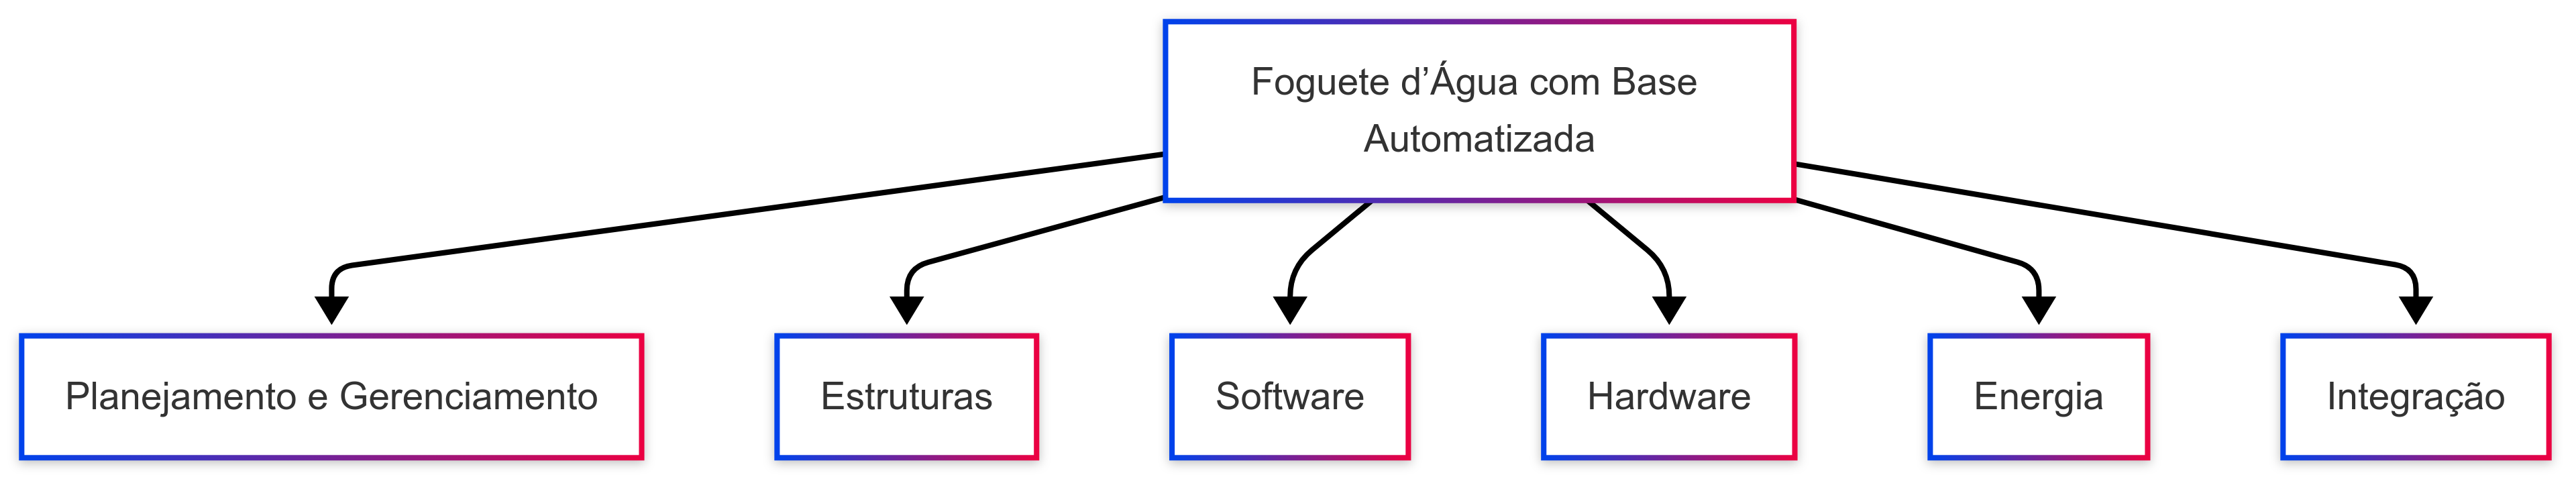
\includegraphics[width=15cm]{figuras/eap_unificado.png}
	\caption{EAP Geral}
	\label{fig_eap_unificado} 
\end{figure}

% --------

\subsection{Planejamento e Gerenciamento}

Este pacote de trabalho contempla os processos de iniciação, planejamento e monitoramento do projeto. Abrange a elaboração do Termo de Abertura do Projeto (TAP), a consolidação da EAP e dos cronogramas setoriais, o planejamento orçamentário, os relatórios de acompanhamento (planejado x realizado) e as atividades de encerramento, como eventos de avaliação SWOT, lições aprendidas e avaliação de desempenho da equipe, conforme a Figura \ref{fig_eap_planejamento}.

\begin{figure}[!h]
	\centering
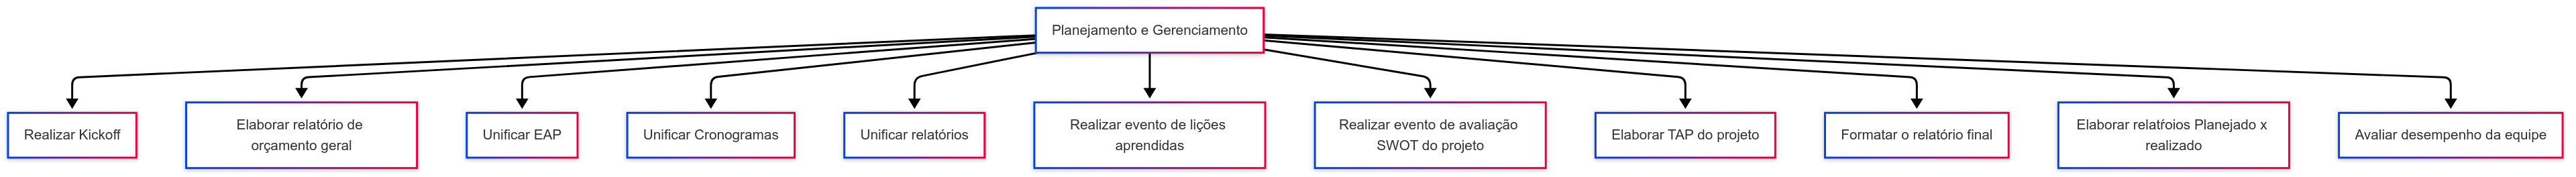
\includegraphics[width=15cm]{figuras/eap_planejamento.png}
	\caption{Pacote de Trabalho 1.1 – Planejamento e Gerenciamento}
	\label{fig_eap_planejamento} 
\end{figure}

\newpage

Eventualmente, o pacote de trabalho de Planejamento e Gerenciamento foi extendido para o modelo de Fluxo de Valor do Produto (VPMN), conforme ilustrado na Figura~\ref{fig_vpmn}. O VPMN é uma abordagem que visa otimizar o fluxo de valor ao longo do ciclo de vida do produto, garantindo que cada etapa agregue valor ao cliente e ao negócio.

\begin{figure}[!h]
	\centering
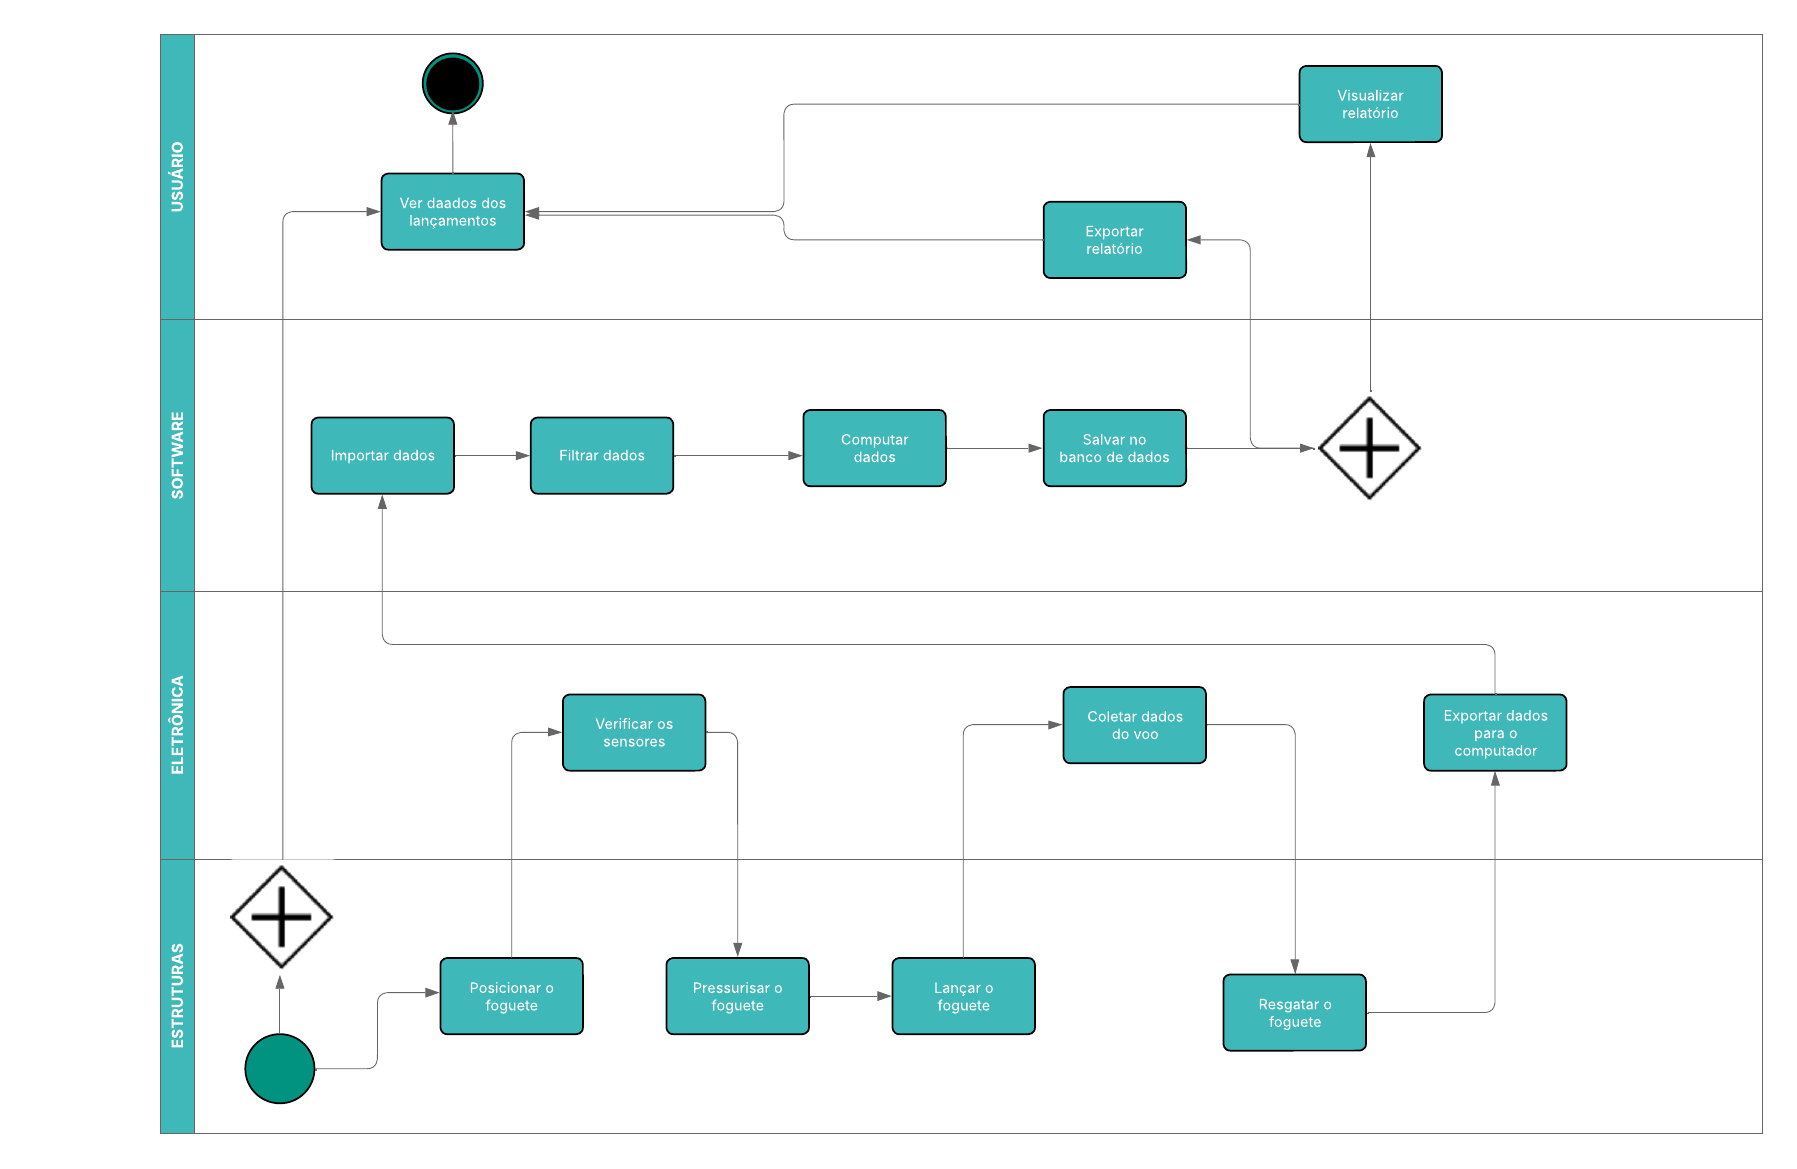
\includegraphics[width=15cm]{figuras/vpmn.png}
	\caption{Pacote de Trabalho 1.1 – VPMN}
	\label{fig_vpmn} 
\end{figure}

% -------------------------------------------------------------------------------------------------------------------------------------------


\section{Casos de Teste}

\subsection*{Testes de Sistema}


\begin{figure}[H]
    \centering
\begin{longtable}{|p{0.2\textwidth}|p{0.7\textwidth}|}
\hline
\multicolumn{2}{|l|}{\textbf{CT01 - Importação de Arquivo JSON Válido}} \\
\hline
\textbf{Tipo} & Teste de sistema \\
\hline
\textbf{Objetivo} & Verificar se o sistema é capaz de importar corretamente um arquivo JSON com dados válidos. \\
\hline
\textbf{Pré-condições} & O sistema deve estar iniciado. Deve haver um arquivo "database.json" com dados completos e corretos no formato esperado.  \\
\hline
\textbf{Procedimentos} & Abrir o sistema. Acessar a funcionalidade "Importar Dados". Selecionar o arquivo "database.json". Confirmar importação. \\
\hline
\textbf{Resultado esperado} & O sistema exibe mensagem de sucesso. Os dados são carregados na interface. Nenhum erro é exibido. \\
\hline
\textbf{Especificação do Reparo} & Verificar se o parser JSON está tratando corretamente os campos esperados. Validar se o caminho de acesso ao arquivo está correto. Corrigir o tratamento de erros silenciosos na importação. \\
\hline
\textbf{Resultado Após Reparo} & O sistema importa corretamente arquivos válidos e exibe os dados esperados. Teste é reexecutado e aprovado. \\
\hline
\end{longtable}
\caption{Caso de Teste 01 - Importação de Arquivo JSON Válido}
\label{fig_ct01_importacao_json_valido}
\end{figure}

\begin{figure}[H]
    \centering
\begin{longtable}{|p{0.2\textwidth}|p{0.7\textwidth}|}
\hline
\multicolumn{2}{|l|}{\textbf{CT02 - Importação de JSON com campos ausentes}} \\
\hline
\textbf{Tipo} & Sistema \\
\hline
\textbf{Objetivo} & Verificar o comportamento do sistema ao importar registros incompletos. \\
\hline
\textbf{Pré-condições} & Arquivo "dados\_incompletos.json" com campos obrigatórios ausentes. \\
\hline
\textbf{Procedimentos} & Acessar "Importar Dados". Selecionar "dados\_incompletos.json". Confirmar importação. \\
\hline
\textbf{Resultado esperado} & Sistema identifica e ignora os registros inválidos. \\
\hline
\textbf{Especificação do Reparo} & Adicionar validação de campos obrigatórios durante o parsing. \\
\hline
\textbf{Resultado após Reparo} & Registros incompletos tratados corretamente. \\
\hline
\end{longtable}
\caption{Caso de Teste 02 - Importação de JSON com campos ausentes}
\label{fig_ct02_importacao_json_campos_ausentes}
\end{figure}

\begin{figure}[H]
    \centering
\begin{longtable}{|p{0.2\textwidth}|p{0.7\textwidth}|}
\hline
\multicolumn{2}{|l|}{\textbf{CT03 - Importação de formato inválido}} \\
\hline
\textbf{Tipo} & Sistema \\
\hline
\textbf{Objetivo} & Garantir que o sistema rejeita arquivos com extensão JSON mas conteúdo inválido (ex: CSV). \\
\hline
\textbf{Pré-condições} & Arquivo "dados\_errados.json" contendo dados CSV. \\
\hline
\textbf{Procedimentos} & Tentar importar "dados\_errados.json". \\
\hline
\textbf{Resultado esperado} & Mensagem de erro de formato exibida. \\
\hline
\textbf{Especificação do Reparo} & Validar estrutura JSON no momento da importação. \\
\hline
\textbf{Resultado após Reparo} & Sistema rejeita corretamente arquivos malformados. \\
\hline
\end{longtable}
\caption{Caso de Teste 03 - Importação de formato inválido}
\label{fig_ct03_importacao_formato_invalido}
\end{figure}

\begin{figure}[H]
    \centering
\begin{longtable}{|p{0.2\textwidth}|p{0.7\textwidth}|}
\hline
\multicolumn{2}{|l|}{\textbf{CT05 - Exportação de Dados para CSV}} \\
\hline
\textbf{Tipo} & Sistema \\
\hline
\textbf{Objetivo} & Garantir que os dados processados sejam exportados corretamente para CSV. \\
\hline
\textbf{Pré-condições} & Dados processados e disponíveis na interface. \\
\hline
\textbf{Procedimentos} & Clicar em "Exportar Dados".  Selecionar "Formato CSV".  Salvar arquivo.  \\
\hline
\textbf{Resultado esperado} & Arquivo CSV é gerado com os dados exibidos. \\
\hline
\textbf{Especificação do Reparo} & Corrigir função de exportação e formatação de colunas. \\
\hline
\textbf{Resultado após Reparo} & Arquivo CSV correto é gerado. \\
\hline
\end{longtable}
\caption{Caso de Teste 05 - Exportação de Dados para CSV}
\label{fig_ct05_exportacao_dados_csv}
\end{figure}

\begin{figure}[H]
    \centering
\begin{longtable}{|p{0.2\textwidth}|p{0.7\textwidth}|}
\hline
\multicolumn{2}{|l|}{\textbf{CT06 – Responsividade da Interface}} \\
\hline
\textbf{Tipo} & Sistema \\
\hline
\textbf{Objetivo} & Verificar o comportamento da interface em diferentes resoluções da tela. \\
\hline
\textbf{Pré-condições} & Sistema em execução. \\
\hline
\textbf{Procedimentos} & Acessar a aplicação em diferentes tamanhos de tela. Navegar pelas funcionalidades. \\
\hline
\textbf{Resultado esperado} & Componentes se ajustam corretamente, sem sobreposições ou corte. \\
\hline
\textbf{Especificação do Reparo} & Ajustar responsividade. \\
\hline
\textbf{Resultado após Reparo} & Interface se adapta corretamente a todas as resoluções testadas. \\
\hline
\end{longtable}
\caption{Caso de Teste 06 - Responsividade da Interface}
\label{fig_ct06_responsividade_interface}
\end{figure}

\begin{figure}[H]
    \centering
\begin{longtable}{|p{0.2\textwidth}|p{0.7\textwidth}|}
\hline
\multicolumn{2}{|l|}{\textbf{CT07 - Validação dos sensores no lançamento do foguete}} \\
\hline
\textbf{Tipo} & Sistema \\
\hline
\textbf{Objetivo} & Verificar se os dados coletados pelos sensores (pressão, ângulo, massa) estão sendo corretamente lidos e registrados no início do lançamento. \\
\hline
\textbf{Pré-condições} & Sistema embarcado ligado.  Foguete pronto para lançamento.  Todos os sensores conectados corretamente. \\
\hline
\textbf{Procedimentos} & Ligar o sistema de aquisição de dados.  Acionar o lançamento do foguete.  Verificar os dados registrados pelos sensores na interface de análise. \\
\hline
\textbf{Resultado Esperado} & Os dados de pressão, ângulo e massa devem ser capturados corretamente, sem valores nulos ou inconsistentes, e armazenados no JSON gerado. \\
\hline
\textbf{Especificação do Reparo} & Verificar conexões físicas dos sensores, calibrar sensores com valores reais, corrigir erros de leitura no firmware. \\
\hline
\textbf{Resultado Após Reparo} & Os sensores coletam os dados de forma correta e os valores são exibidos e armazenados conforme esperado. \\
\hline
\end{longtable}
\caption{Caso de Teste 07 - Validação dos sensores no lançamento do foguete}
\label{fig_ct07_validacao_sensores_lancamento_foguete}
\end{figure}

\begin{figure}[H]
    \centering
\begin{longtable}{|p{0.2\textwidth}|p{0.7\textwidth}|}
\hline
\multicolumn{2}{|l|}{\textbf{CT08 - Funcionamento do mecanismo de lançamento}} \\
\hline
\textbf{Tipo} & Sistema \\
\hline
\textbf{Objetivo} & Verificar o funcionamento do mecanismo de lançamento. \\
\hline
\textbf{Pré-condições} & Sistema embarcado ligado.  Foguete carregado com água e pressurizado. \\
\hline
\textbf{Procedimentos} & Acionar o sistema de lançamento via interface.  Observar o funcionamento do atuador eletromecânico. \\
\hline
\textbf{Resultado Esperado} & O foguete deve ser lançado automaticamente após o comando, sem falhas mecânicas ou atraso. \\
\hline
\textbf{Especificação do Reparo} & Verificar fiação, tensão e código do acionamento do atuador. \\
\hline
\textbf{Resultado Após Reparo} & Atuador funciona corretamente e o foguete é lançado de forma imediata e estável. \\
\hline
\end{longtable}
\caption{Caso de Teste 08 - Funcionamento do mecanismo de lançamento}
\label{fig_ct08_funcionamento_mecanismo_lancamento}
\end{figure}

\subsection*{Testes de Integração}

\begin{figure}[H]
    \centering
\begin{longtable}{|p{0.2\textwidth}|p{0.7\textwidth}|}
\hline
\multicolumn{2}{|l|}{\textbf{CT04 - Geração dos gráficos}} \\
\hline
\textbf{Tipo} & Integração \\
\hline
\textbf{Objetivo} & Verificar se o sistema gera corretamente o gráfico de altitude após a importação dos dados. \\
\hline
\textbf{Pré-condições} & Dados válidos já importados. \\
\hline
\textbf{Procedimentos} & Acessar a interface de visualização de gráficos. \\
\hline
\textbf{Resultado Esperado} & Gráfico exibido com dados coerentes. \\
\hline
\textbf{Especificação do Reparo} & Ajustar lógica de plotagem ou eixos do gráfico. \\
\hline
\textbf{Resultado após Reparo} & Gráfico é exibido corretamente. \\
\hline
\end{longtable}
\caption{Caso de Teste 04 - Geração dos gráficos}
\label{fig_ct04_geracao_graficos}
\end{figure}

\begin{figure}[H]
    \centering
\begin{longtable}{|p{0.2\textwidth}|p{0.7\textwidth}|}
\hline
\multicolumn{2}{|l|}{\textbf{CT24 - Integração entre ESP32 e Sensores}} \\
\hline
\textbf{Tipo} & Integração \\
\hline
\textbf{Objetivo} & Verificar se os sensores (pressão, ângulo, massa) estão integrados corretamente ao ESP32 e geram dados coerentes. \\
\hline
\textbf{Pré-condições} & Firmware embarcado finalizado.  Todos os sensores ligados ao ESP32. \\
\hline
\textbf{Procedimentos} & Iniciar sistema embarcado.  Coletar dados em tempo real dos sensores.  Verificar se os dados são salvos e transmitidos corretamente. \\
\hline
\textbf{Resultado esperado} & Leituras coerentes e disponíveis para transmissão e armazenamento. \\
\hline
\textbf{Especificação do Reparo} & Verificar drivers de sensores, conexões físicas e timing de leitura. \\
\hline
\textbf{Resultado após Reparo} & Sistema lê e integra dados sem falhas ou atrasos. \\
\hline
\end{longtable}
\caption{Caso de Teste 24 - Integração entre ESP32 e Sensores}
\label{fig_ct24_integracao_esp32_sensores}
\end{figure}

\begin{figure}[H]
    \centering
\begin{longtable}{|p{0.2\textwidth}|p{0.7\textwidth}|}
\hline
\multicolumn{2}{|l|}{\textbf{CT25 - Integração entre Foguete e Base (LoRa)}} \\
\hline
\textbf{Tipo} & Integração \\
\hline
\textbf{Objetivo} & Garantir que os dados gerados no voo são transmitidos e recebidos pela base sem perdas relevantes. \\
\hline
\textbf{Pré-condições} & Firmware de transmissão e recepção finalizado.  Antenas e módulos LoRa funcionando. \\
\hline
\textbf{Procedimentos} & Iniciar voo de teste (ou simulação).  Observar dados transmitidos em tempo real (base recebe JSON).  Comparar dados recebidos com dados salvos no MicroSD. \\
\hline
\textbf{Resultado esperado} & Dados coerentes e transmissão confiável. \\
\hline
\textbf{Especificação do Reparo} & Ajustar parâmetros LoRa (velocidade, potência) e revisar firmware. \\
\hline
\textbf{Resultado após Reparo} & Comunicação estável e sem falhas críticas. \\
\hline
\end{longtable}
\caption{Caso de Teste 25 - Integração entre Foguete e Base (LoRa)}
\label{fig_ct25_integracao_foguete_base_lora}
\end{figure}

\begin{figure}[H]
    \centering
\begin{longtable}{|p{0.2\textwidth}|p{0.7\textwidth}|}
\hline
\multicolumn{2}{|l|}{\textbf{CT26 - Integração Energética – Estabilidade no Sistema Completo}} \\
\hline
\textbf{Tipo} & Integração \\
\hline
\textbf{Objetivo} & Verificar se a fonte de energia dimensionada suporta o consumo de todos os componentes ao mesmo tempo. \\
\hline
\textbf{Pré-condições} & Sistema montado com todos os sensores e atuadores ativos.  Fonte de energia de 3,3 V e corrente maior que 300\,mA. \\
\hline
\textbf{Procedimentos} & Ligar todos os módulos simultaneamente (ex: pressão, atuadores, display, etc.).  Observar estabilidade de tensão e corrente durante 30 segundos.  Verificar se não ocorrem quedas ou falhas. \\
\hline
\textbf{Resultado esperado} & Tensão estável ($\pm 6\%$) e corrente $\le$ capacidade máxima ($300$)mA. \\
\hline
\textbf{Especificação do Reparo} & Substituir a fonte por uma de maior capacidade ou revisar fiação. \\
\hline
\textbf{Resultado após Reparo} & Sistema opera sem oscilações ou falhas de alimentação. \\
\hline
\end{longtable}
\caption{Caso de Teste 26 - Integração Energética – Estabilidade no Sistema Completo}
\label{fig_ct26_integracao_energetica_estabilidade_sistema_completo}
\end{figure}

\subsection*{Testes de Unidade}

\begin{figure}[H]
    \centering
\begin{longtable}{|p{0.2\textwidth}|p{0.7\textwidth}|}
\hline
\multicolumn{2}{|l|}{\textbf{CT09 - Parser de JSON Válido}} \\
\hline
\textbf{Tipo} & Unidade \\
\hline
\textbf{Objetivo} & Verificar leitura de JSON com dados completos. \\
\hline
\textbf{Pré-condições} & Função de parser implementada e disponível no ambiente de desenvolvimento.  Arquivo de teste válido com dados completos. \\
\hline
\textbf{Procedimentos} & Rodar função de parser diretamente com arquivo de teste válido.  Verificar se estrutura retornada está correta. \\
\hline
\textbf{Resultado esperado} & Dados carregados na memória, sem exceções. \\
\hline
\textbf{Especificação do Reparo} & Revisar lógica de leitura e formatação do JSON.  Corrigir tratamento de exceções ou formatação incorreta. \\
\hline
\textbf{Resultado após Reparo} & Parser reconhece corretamente arquivos válidos e gera a estrutura esperada sem exceções. \\
\hline
\end{longtable}
\caption{Caso de Teste 09 - Parser de JSON Válido}
\label{fig_ct09_parser_json_valido}
\end{figure}

\begin{figure}[H]
    \centering
\begin{longtable}{|p{0.2\textwidth}|p{0.7\textwidth}|}
\hline
\multicolumn{2}{|l|}{\textbf{CT10 - Parser de JSON com Campos Ausentes}} \\
\hline
\textbf{Tipo} & Unidade \\
\hline
\textbf{Objetivo} & Garantir tratamento de dados incompletos. \\
\hline
\textbf{Pré-condições} & Função de parser em funcionamento.  JSON de teste com campos ausentes. \\
\hline
\textbf{Procedimentos} &  Rodar parser com JSON que tenha campos ausentes.  Verificar se registros inválidos são removidos. \\
\hline
\textbf{Resultado esperado} & Retorno apenas dos registros completos. \\
\hline
\textbf{Especificação do Reparo} & Corrigir verificação de campos obrigatórios.  Implementar descartes controlados de registros inválidos. \\
\hline
\textbf{Resultado após Reparo} & Parser filtra registros incompletos sem falhas. \\
\hline
\end{longtable}
\caption{Caso de Teste 10 - Parser de JSON com Campos Ausentes}
\label{fig_ct10_parser_json_campos_ausentes}
\end{figure}

\begin{figure}[H]
    \centering
\begin{longtable}{|p{0.2\textwidth}|p{0.7\textwidth}|}
\hline
\multicolumn{2}{|l|}{\textbf{CT27 - Parser de JSON com Dados Absurdos}} \\
\hline
\textbf{Tipo} & Unidade \\
\hline
\textbf{Objetivo} & Verificar descarte de dados absurdos (ex: altitude negativa). \\
\hline
\textbf{Pré-condições} & Função de validação em funcionamento.  Lista de dados brutos com registros absurdos. \\
\hline
\textbf{Procedimentos} & Rodar função de validação com lista de dados brutos.  Observar se registros absurdos são filtrados. \\
\hline
\textbf{Resultado esperado} & Lista resultante sem registros absurdos. \\
\hline
\textbf{Especificação do Reparo} & Corrigir regra de validação de campos.  Implementar descarte de dados absurdos. \\
\hline
\textbf{Resultado após Reparo} & Função remove corretamente dados absurdos sem impactar o restante. \\
\hline
\end{longtable}
\caption{Caso de Teste 27 - Parser de JSON com Dados Absurdos}
\label{fig_ct27_parser_json_dados_absurdos}
\end{figure}

\begin{figure}[H]
    \centering
\begin{longtable}{|p{0.2\textwidth}|p{0.7\textwidth}|}
\hline
\multicolumn{2}{|l|}{\textbf{CT11 - Aplicação de Filtro de Média Móvel}} \\
\hline
\textbf{Tipo} & Unidade \\
\hline
\textbf{Objetivo} & Verificar aplicação correta de filtro. \\
\hline
\textbf{Pré-condições} & Função de filtro implementada.  Dados de teste com ruído disponíveis.  \\
\hline
\textbf{Procedimentos} & Rodar função de filtro com dados de teste (com ruído).  Comparar saída com valores esperados (média móvel conhecida).  \\
\hline
\textbf{Resultado esperado} & Dados suavizados sem distorção indevida. \\
\hline
\textbf{Especificação do Reparo} & Ajustar janela ou lógica de média móvel.  Corrigir cálculos que gerem resultados errados. \\
\hline
\textbf{Resultado após Reparo} & Filtro suaviza corretamente os dados e remove ruídos. \\
\hline
\end{longtable}
\caption{Caso de Teste 11 - Aplicação de Filtro de Média Móvel}
\label{fig_ct11_filtro_media_movel}
\end{figure}

\begin{figure}[H]
    \centering
\begin{longtable}{|p{0.2\textwidth}|p{0.7\textwidth}|}
\hline
\multicolumn{2}{|l|}{\textbf{CT12 - Exportação de Dados para CSV}} \\
\hline
\textbf{Tipo} & Unidade \\
\hline
\textbf{Objetivo} & Validar formatação e consistência do CSV. \\
\hline
\textbf{Pré-condições} & Função de exportação implementada e em funcionamento.  Dados em memória para exportação. \\
\hline
\textbf{Procedimentos} & Rodar função de exportação com dados em memória.  Abrir CSV e verificar cabeçalhos, formato e integridade dos dados. \\
\hline
\textbf{Resultado esperado} & Arquivo CSV gerado sem erros. \\
\hline
\textbf{Especificação do Reparo} & Corrigir escrita do arquivo CSV (formato e separadores).  Ajustar cabeçalhos e ordem de dados. \\
\hline
\textbf{Resultado após Reparo} & CSV exportado corretamente e sem inconsistências. \\
\hline
\end{longtable}
\caption{Caso de Teste 12 - Exportação de Dados para CSV}
\label{fig_ct12_exportacao_dados_csv}
\end{figure}

\begin{figure}[H]
    \centering
\begin{longtable}{|p{0.2\textwidth}|p{0.7\textwidth}|}
\hline
\multicolumn{2}{|l|}{\textbf{CT13 - Geração de gráfico}} \\
\hline
\textbf{Tipo} & Unidade \\
\hline
\textbf{Objetivo} & Validar coerência visual dos gráficos gerados. \\
\hline
\textbf{Pré-condições} & Função de geração de gráficos implementada.  Dados de teste consistentes.  \\
\hline
\textbf{Procedimentos} & Rodar função de geração de gráficos com dados de teste.  Conferir se gráfico está correto visualmente e numericamente.  \\
\hline
\textbf{Resultado esperado} & Gráfico gerado com dados coerentes e layout adequado. \\
\hline
\textbf{Especificação do Reparo} &  Ajustar lógica de plotagem (eixos e escalas).  Corrigir erros de indexação de dados.  \\
\hline
\textbf{Resultado após Reparo} & Gráficos exibem dados de forma coerente e confiável. \\
\hline
\end{longtable}
\caption{Caso de Teste 13 - Geração de gráfico}
\label{fig_ct13_geracao_grafico}
\end{figure}

\begin{figure}[H]
    \centering
\begin{longtable}{|p{0.2\textwidth}|p{0.7\textwidth}|}
\hline
\multicolumn{2}{|l|}{\textbf{CT14 - Validação do Sensor MPX5700 (Pressão)}} \\
\hline
\textbf{Tipo} & Unidade (hardware/embarcado) \\
\hline
\textbf{Objetivo} & Garantir leitura coerente da pressão durante carregamento. \\
\hline
\textbf{Pré-condições} & Sistema embarcado ligado e calibrado. \\
\hline
\textbf{Procedimentos} &  Pressurizar gradualmente a câmara.  Ler valores do sensor de pressão.  Comparar com medidor externo confiável.  \\
\hline
\textbf{Resultado esperado} & Leituras consistentes, sem desvios bruscos. \\
\hline
\textbf{Especificação do Reparo} & Calibrar sensor ou corrigir conversão no firmware. \\
\hline
\textbf{Resultado após Reparo} & Leituras de pressão confiáveis e coerentes. \\
\hline
\end{longtable}
\caption{Caso de Teste 14 - Validação do Sensor MPX5700 (Pressão)}
\label{fig_ct14_validacao_sensor_mpx5700}
\end{figure}

\begin{figure}[H]
    \centering
\begin{longtable}{|p{0.2\textwidth}|p{0.7\textwidth}|}
\hline
\multicolumn{2}{|l|}{\textbf{CT15 - Validação do Sensor MPU-6500 (Acelerômetro)}} \\
\hline
\textbf{Tipo} & Unidade (hardware/embarcado) \\
\hline
\textbf{Objetivo} & Verificar se a leitura de aceleração está coerente com o movimento. \\
\hline
\textbf{Pré-condições} & Sistema embarcado funcional. \\
\hline
\textbf{Procedimentos} &  Simular movimentos suaves e bruscos do foguete.  Observar leituras de aceleração.  \\
\hline
\textbf{Resultado esperado} & Dados refletem as variações reais de movimento. \\
\hline
\textbf{Especificação do Reparo} & Calibrar sensor e revisar código de leitura. \\
\hline
\textbf{Resultado após Reparo} & Sensor reporta acelerações reais de forma confiável. \\
\hline
\end{longtable}
\caption{Caso de Teste 15 - Validação do Sensor MPU-6500 (Acelerômetro)}
\label{fig_ct15_validacao_sensor_mpu6500}
\end{figure}

\begin{figure}[H]
    \centering
\begin{longtable}{|p{0.2\textwidth}|p{0.7\textwidth}|}
\hline
\multicolumn{2}{|l|}{\textbf{CT16 - Leitura do Sensor de Massa}} \\
\hline
\textbf{Tipo} & Unidade \\
\hline
\textbf{Objetivo} & Garantir leitura correta da massa do foguete antes do lançamento. \\
\hline
\textbf{Pré-condições} &  Sensor de massa calibrado.  Massa real conhecida.  \\
\hline
\textbf{Procedimentos} &  Colocar o foguete com massa conhecida na plataforma.  Ler os dados da célula de carga via firmware.  Comparar leitura com massa real medida em balança.  \\
\hline
\textbf{Resultado esperado} & Erro máximo aceitável ($\pm 10$g). \\
\hline
\textbf{Especificação do Reparo} & Verificar calibração e conexão do sensor. Corrigir leituras incorretas no firmware. \\
\hline
\textbf{Resultado após Reparo} & Leitura de massa consistente com o valor real. \\
\hline
\end{longtable}
\caption{Caso de Teste 16 - Leitura do Sensor de Massa}
\label{fig_ct16_leitura_sensor_massa}
\end{figure}

\begin{figure}[H]
    \centering
\begin{longtable}{|p{0.2\textwidth}|p{0.7\textwidth}|}
\hline
\multicolumn{2}{|l|}{\textbf{CT17 - Validação do Dimensionamento Energético}} \\
\hline
\textbf{Tipo} & Unidade \\
\hline
\textbf{Objetivo} & Verificar se o fornecimento de energia atende ao consumo calculado com margem de segurança. \\
\hline
\textbf{Pré-condições} &  Sistema embarcado montado com todos os sensores e atuadores conectados.  Fonte de alimentação dimensionada.  \\
\hline
\textbf{Procedimentos} &  Ligar o sistema completo.  Monitorar tensão e corrente durante 30 segundos.  Verificar se a tensão permanece estável.  Verificar se a corrente total está dentro da faixa de consumo.  \\
\hline
\textbf{Resultado esperado} & Sistema opera sem quedas de tensão ou falhas de alimentação. \\
\hline
\textbf{Especificação do Reparo} & Substituir fonte de alimentação ou ajustar conexões elétricas. \\
\hline
\textbf{Resultado após Reparo} & Sistema estável durante todo o tempo de operação. \\
\hline
\end{longtable}
\caption{Caso de Teste 17 - Validação do Dimensionamento Energético}
\label{fig_ct17_validacao_dimensionamento_energetico}
\end{figure}

\begin{figure}[H]
    \centering
\begin{longtable}{|p{0.2\textwidth}|p{0.7\textwidth}|}
\hline
\multicolumn{2}{|l|}{\textbf{CT18 - Validação do Atuador - Válvula Solenóide}} \\
\hline
\textbf{Tipo} & Unidade \\
\hline
\textbf{Objetivo} & Verificar se a válvula solenóide abre/fecha corretamente sob comando. \\
\hline
\textbf{Pré-condições} &  Sistema embarcado funcional.  Compressor e pressão dentro do esperado.  \\
\hline
\textbf{Procedimentos} &  Acionar a válvula via relé (comando direto no firmware).  Observar se há liberação/fechamento imediato de ar.  \\
\hline
\textbf{Resultado esperado} & Válvula responde rapidamente ao comando sem falhas. \\
\hline
\textbf{Especificação do Reparo} & Verificar conexões elétricas e integridade do relé. \\
\hline
\textbf{Resultado após Reparo} & Válvula abre/fecha conforme esperado. \\
\hline
\end{longtable}
\caption{Caso de Teste 18 - Validação do Atuador - Válvula Solenóide}
\label{fig_ct18_validacao_atuador_valvula_solenoide}
\end{figure}

\begin{figure}[H]
    \centering
\begin{longtable}{|p{0.2\textwidth}|p{0.7\textwidth}|}
\hline
\multicolumn{2}{|l|}{\textbf{CT19 - Validação do Atuador - Compressor}} \\
\hline
\textbf{Tipo} & Unidade \\
\hline
\textbf{Objetivo} & Verificar funcionamento do compressor 12 V durante a fase de pressurização. \\
\hline
\textbf{Pré-condições} & Sistema montado e conectado ao relé. \\
\hline
\textbf{Procedimentos} &  Enviar comando para ativar compressor.  Observar operação estável e sem superaquecimento.  \\
\hline
\textbf{Resultado esperado} & Compressor enche a câmara e atinge pressão esperada. \\
\hline
\textbf{Especificação do Reparo} & Verificar tensão de alimentação, relé e conexões físicas. \\
\hline
\textbf{Resultado após Reparo} & Compressor opera normalmente sem falhas. \\
\hline
\end{longtable}
\caption{Caso de Teste 19 - Validação do Atuador - Compressor}
\label{fig_ct19_validacao_atuador_compressor}
\end{figure}

\begin{figure}[H]
    \centering
\begin{longtable}{|p{0.2\textwidth}|p{0.7\textwidth}|}
\hline
\multicolumn{2}{|l|}{\textbf{CT20 - Validação do Atuador - Buzzer}} \\
\hline
\textbf{Tipo} & Unidade \\
\hline
\textbf{Objetivo} & Verificar se o buzzer emite contagem regressiva sonora. \\
\hline
\textbf{Pré-condições} & Firmware com contagem regressiva implementada. \\
\hline
\textbf{Procedimentos} &  Acionar comando de contagem regressiva.  Observar sequência de sons de 10 a 0.  \\
\hline
\textbf{Resultado esperado} & Sons nítidos e no tempo correto. \\
\hline
\textbf{Especificação do Reparo} & Verificar ligação do buzzer e ajuste do firmware. \\
\hline
\textbf{Resultado após Reparo} & Contagem sonora clara e funcional. \\
\hline
\end{longtable}
\caption{Caso de Teste 20 - Validação do Atuador - Buzzer}
\label{fig_ct20_validacao_atuador_buzzer}
\end{figure}

\begin{figure}[H]
    \centering
\begin{longtable}{|p{0.2\textwidth}|p{0.7\textwidth}|}
\hline
\multicolumn{2}{|l|}{\textbf{CT21 - Validação da Conectividade LoRa (RFM95W)}} \\
\hline
\textbf{Tipo} & Unidade \\
\hline
\textbf{Objetivo} & Garantir comunicação confiável entre ESP32 da base e do foguete. \\
\hline
\textbf{Pré-condições} & Ambientes de teste prontos (foguete e base). \\
\hline
\textbf{Procedimentos} &  Ligar ambos os dispositivos.  Iniciar transmissão de dados de teste do foguete para a base.  Observar recepção sem perdas significativas.  \\
\hline
\textbf{Resultado esperado} & Dados JSON recebidos sem interrupções relevantes. \\
\hline
\textbf{Especificação do Reparo} & Ajustar parâmetros de transmissão ou antenas. \\
\hline
\textbf{Resultado após Reparo} & Comunicação estável e confiável via LoRa. \\
\hline
\end{longtable}
\caption{Caso de Teste 21 - Validação da Conectividade LoRa (RFM95W)}
\label{fig_ct21_validacao_conectividade_lora}
\end{figure}

\begin{figure}[H]
    \centering
\begin{longtable}{|p{0.2\textwidth}|p{0.7\textwidth}|}
\hline
\multicolumn{2}{|l|}{\textbf{CT22 - Validação do Módulo de Armazenamento MicroSD}} \\
\hline
\textbf{Tipo} & Unidade \\
\hline
\textbf{Objetivo} & Garantir que os dados de voo são salvos corretamente no cartão. \\
\hline
\textbf{Pré-condições} & Sistema do foguete funcional e MicroSD inserido. \\
\hline
\textbf{Procedimentos} &  Iniciar simulação de voo.  Salvar dados de sensores no MicroSD.  Remover cartão e abrir no computador.  \\
\hline
\textbf{Resultado esperado} & Arquivo JSON salvo e legível. \\
\hline
\textbf{Especificação do Reparo} & Verificar comandos de escrita no firmware e integridade do MicroSD. \\
\hline
\textbf{Resultado após Reparo} & Dados salvos corretamente e legíveis. \\
\hline
\end{longtable}
\caption{Caso de Teste 22 - Validação do Módulo de Armazenamento MicroSD}
\label{fig_ct22_validacao_modulo_armazenamento_microsd}
\end{figure}

\begin{figure}[H]
    \centering
\begin{longtable}{|p{0.2\textwidth}|p{0.7\textwidth}|}
\hline
\multicolumn{2}{|l|}{\textbf{CT23 - Validação do Display LCD 16x4}} \\
\hline
\textbf{Tipo} & Unidade \\
\hline
\textbf{Objetivo} & Verificar exibição correta da contagem visual de 10 a 0. \\
\hline
\textbf{Pré-condições} & Display conectado e inicializado. \\
\hline
\textbf{Procedimentos} & Acionar contagem regressiva no firmware.  Observar exibição da contagem no display.  \\
\hline
\textbf{Resultado esperado} & Dígitos exibidos sem falhas ou cortes. \\
\hline
\textbf{Especificação do Reparo} & Ajustar comunicação I2C e revisão do código. \\
\hline
\textbf{Resultado após Reparo} & Contagem exibida de forma clara e precisa. \\
\hline
\end{longtable}
\caption{Caso de Teste 23 - Validação do Display LCD 16x4}
\label{fig_ct23_validacao_display_lcd}
\end{figure}


% -----------------

\subsection{Estruturas}

Responsável pela modelagem e construção da fuselagem do foguete e da base física de lançamento. Este pacote inclui atividades como elaboração de desenhos técnicos em CAD, levantamento de materiais, montagem estrutural, e realização de experimentos e testes de integração estrutural. Também contempla a avaliação do desempenho de fornecedores, conforme ilustrado na Figura \ref{fig_eap_estruturas}.

\begin{figure}[!h]
	\centering
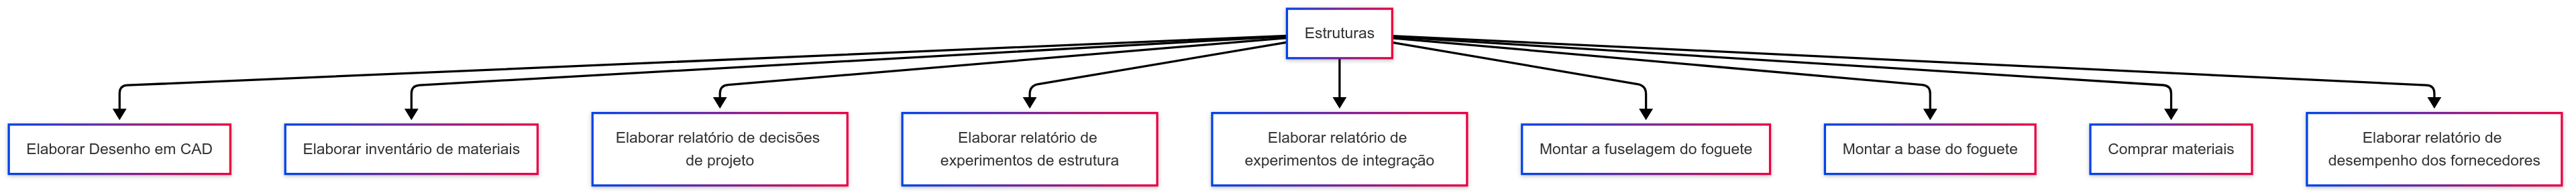
\includegraphics[width=15cm]{figuras/eap_estruturas.png}
	\caption{Pacote de Trabalho 1.2 – Estruturas}
	\label{fig_eap_estruturas} 
\end{figure}

% -------------------------------------------------------------------------------------------------------------------------------------------
% Inicio de Software
% -------------------------------------------------------------------------------------------------------------------------------------------

\subsection{Software}

Este pacote compreende a elicitação de requisitos funcionais e não funcionais, a modelagem da arquitetura do sistema, a construção e testes de software. Inclui ainda a elaboração de diagramas (casos de uso, estados, BPMN), BACKLOG, DER, protótipos navegáveis e relatórios de testes de unidade e integração, conforme apresentado na Figura \ref{fig_eap_software}.

O software desenvolvido tem como principal objetivo coletar, armazenar, processar e apresentar os dados dos lançamentos do foguete de água. Ele permite que os usuários importem os dados registrados pelos sensores do foguete (armazenados em um pendrive ou cartão SD), visualizem esses dados em forma de relatórios e gráficos e mantenham um histórico dos lançamentos realizados.

Além disso, o software possui duas interfaces: uma interface em linha de comando (CLI) voltada para usuários que preferem comandos diretos e uma interface gráfica (GUI) desenvolvida para tornar a visualização dos dados mais acessível e amigável.

\begin{figure}[!h]
	\centering
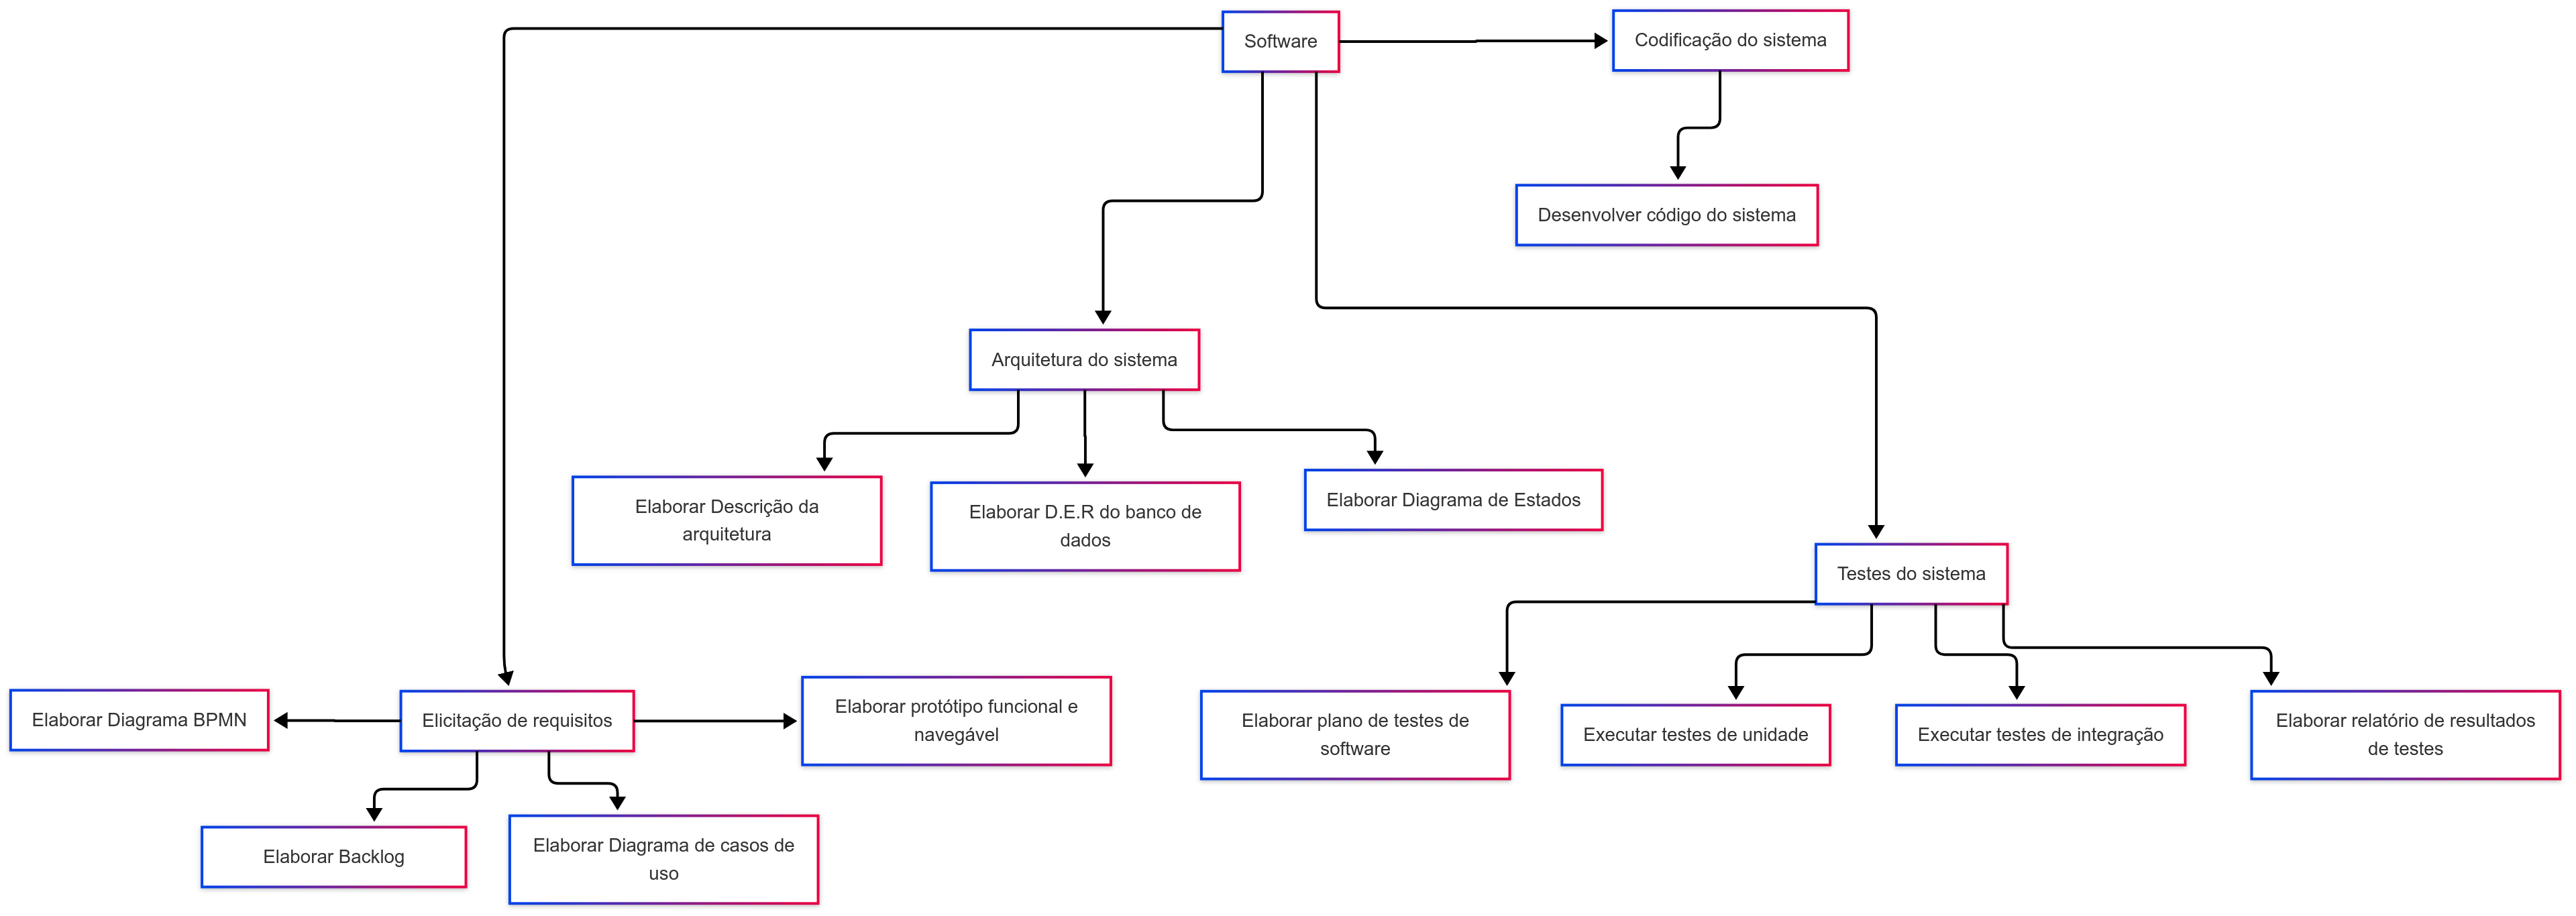
\includegraphics[width=15cm]{figuras/eap_software.png}
	\caption{Pacote de Trabalho 1.3 – Software}
	\label{fig_eap_software} 
\end{figure}

% -------------------------------------------------------------
% MOSCOW
% -------------------------------------------------------------

\begin{samepage}
O pacote MOSCOW é uma técnica de priorização de requisitos que classifica as funcionalidades em quatro categorias: Must have (deve ter), Should have (deveria ter), Could have (poderia ter) e Won't have this time (não terá desta vez). Essa abordagem ajuda a focar no que é essencial para o sucesso do projeto, garantindo que os recursos sejam alocados de forma eficiente. A Figura \ref{tab:requisitos_projeto} ilustra a aplicação dessa técnica no contexto do projeto.

\begin{table}[htpb]
\centering
\scriptsize
\setlength{\tabcolsep}{4pt}
\caption{Tabela de Requisitos do Projeto}
\begin{tabular}{|l|p{8cm}|l|}
\hline
\textbf{ID} & \textbf{DESCRIÇÃO} & \textbf{PRIORIDADE} \\
\hline
RQ01 & Importar dados de voo em JSON de dispositivo externo & Must have \\
\hline
RQ02 & Exibir gráfico de velocidade vertical vs. tempo. & Must have \\
\hline
RQ03 & Exibir gráfico de aceleração vertical vs. tempo. & Must have \\
\hline
RQ04 & Exibir gráfico de dispersão da trajetória no plano X e Y. & Must have \\
\hline
RQ05 & Exibir gráfico de altitude vs. tempo. & Must have \\
\hline
RQ06 & Exibir valores máximos e mínimos de aceleração, velocidade e ângulo. & Should have \\
\hline
RQ07 & Exibir tempo de execução e intervalos de amostragem. & Should have \\
\hline
RQ08 & Exportar dados do voo em JSON. & Must have \\
\hline
RQ09 & Importar arquivos JSON para comparação e simulação. & Must have \\
\hline
RQ10 & Aplicar filtro de média móvel nos dados dos sensores. & Should have \\
\hline
\end{tabular}
\label{tab:requisitos_projeto}
\end{table}

\end{samepage}


% -------------------------------------------------------------
% REQUISITOS NÃO-FUNCIONAIS
% -------------------------------------------------------------

\begin{samepage}
Os requisitos não-funcionais são critérios que definem a qualidade e as restrições do sistema, como desempenho, segurança, usabilidade e portabilidade. Eles são essenciais para garantir que o sistema atenda às expectativas dos usuários e funcione de maneira eficiente em diferentes ambientes. A Tabela \ref{tab:requisitos_nao_funcionais} apresenta os requisitos não-funcionais identificados para o projeto.

\begin{table}[htpb]
\centering
\scriptsize
\setlength{\tabcolsep}{4pt}
\caption{Requisitos Não-Funcionais}
\begin{tabular}{|l|p{11cm}|}
\hline
\textbf{ID} & \textbf{DESCRIÇÃO} \\
\hline
RNF01 & Os dados dos lançamentos devem ser armazenados localmente de forma que não possam ser corrompidos em caso de desligamento inesperado. \\
\hline
RNF02 & O software deve validar a integridade dos arquivos JSON antes de processar os dados. \\
\hline
RNF03 & O software deve ser multiplataforma, funcionando em pelo menos Windows, Linux e MacOS. \\
\hline
RNF04 & Não deve depender de conexão com internet para funcionar. \\
\hline
RNF05 & A geração de relatórios e gráficos não deve exceder 3 segundos para arquivos de até 100 lançamentos. \\
\hline
RNF06 & A interface gráfica (GUI) deve ser intuitiva, com botões claros para importar dados, gerar gráficos e acessar os lançamentos anteriores. \\
\hline
RNF07 & O CLI deve ter comandos simples. \\
\hline
\end{tabular}
\label{tab:requisitos_nao_funcionais}
\end{table}
\end{samepage}

% -------------------------------------------------------------
% CASOS DE USO
% -------------------------------------------------------------

\begin{samepage}

O pacote de Casos de Uso é uma técnica de modelagem que descreve as interações entre os usuários (atores) e o sistema, detalhando como os requisitos funcionais serão atendidos. Os casos de uso ajudam a identificar as funcionalidades essenciais do sistema e a garantir que todas as partes interessadas tenham uma compreensão clara dos objetivos do projeto. A Figura \ref{fig_casos_de_uso} apresenta um exemplo de diagrama de casos de uso utilizado no projeto.
\begin{figure}[!h]
	\centering
	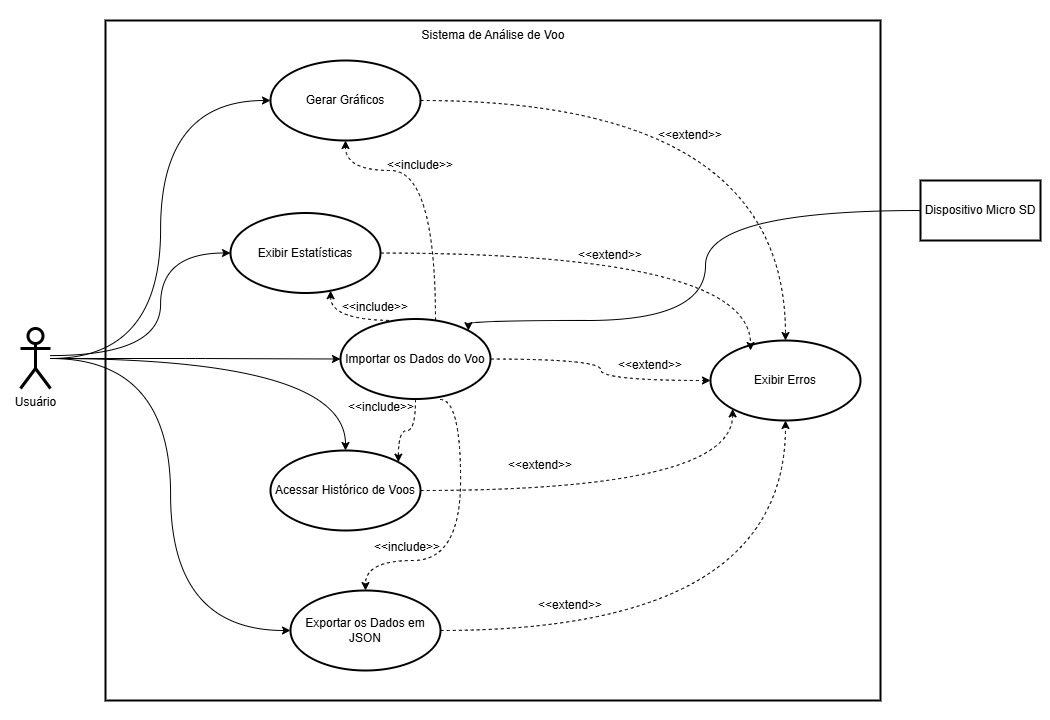
\includegraphics[width=15cm]{figuras/caso_de_uso.png}
	\caption{Pacote de Trabalho 1.3 – Casos de Uso}
	\label{fig_casos_de_uso}
\end{figure}
\end{samepage}

% -------------------------------------------------------------
% DIAGRAMA DE ENTIDADE-RELACIONAMENTO
% -------------------------------------------------------------

\begin{samepage}

O Diagrama de Entidade-Relacionamento (DER) é uma técnica de modelagem de dados que representa as entidades do sistema e os relacionamentos entre elas. É fundamental para a construção do banco de dados e para garantir que os dados sejam organizados de forma eficiente. A Figura \ref{fig_der} ilustra um exemplo de DER utilizado no projeto.

\begin{figure}[!h]
	\centering
	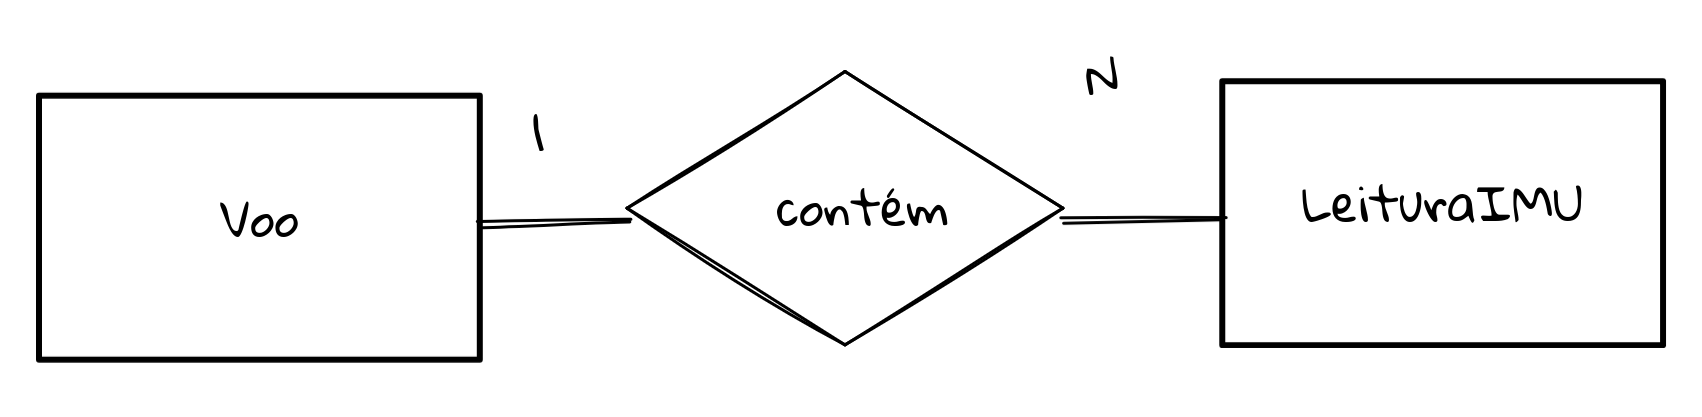
\includegraphics[width=15cm]{figuras/der.png}
	\caption{Pacote de Trabalho 1.3 – Diagrama de Entidade-Relacionamento}
	\label{fig_der}
\end{figure}

Após isso, podemos modelar os atributos de cada entidade, conforme os dados que receberemos da ERP32, que calculará movimentos de unidade de medição inercial pelo sensor de 6 eixos, como o acelerômetro e o giroscópio. A Figura \ref{fig_atributos} apresenta um exemplo de atributos modelados para as entidades do sistema.

\begin{figure}[!h]
	\centering
	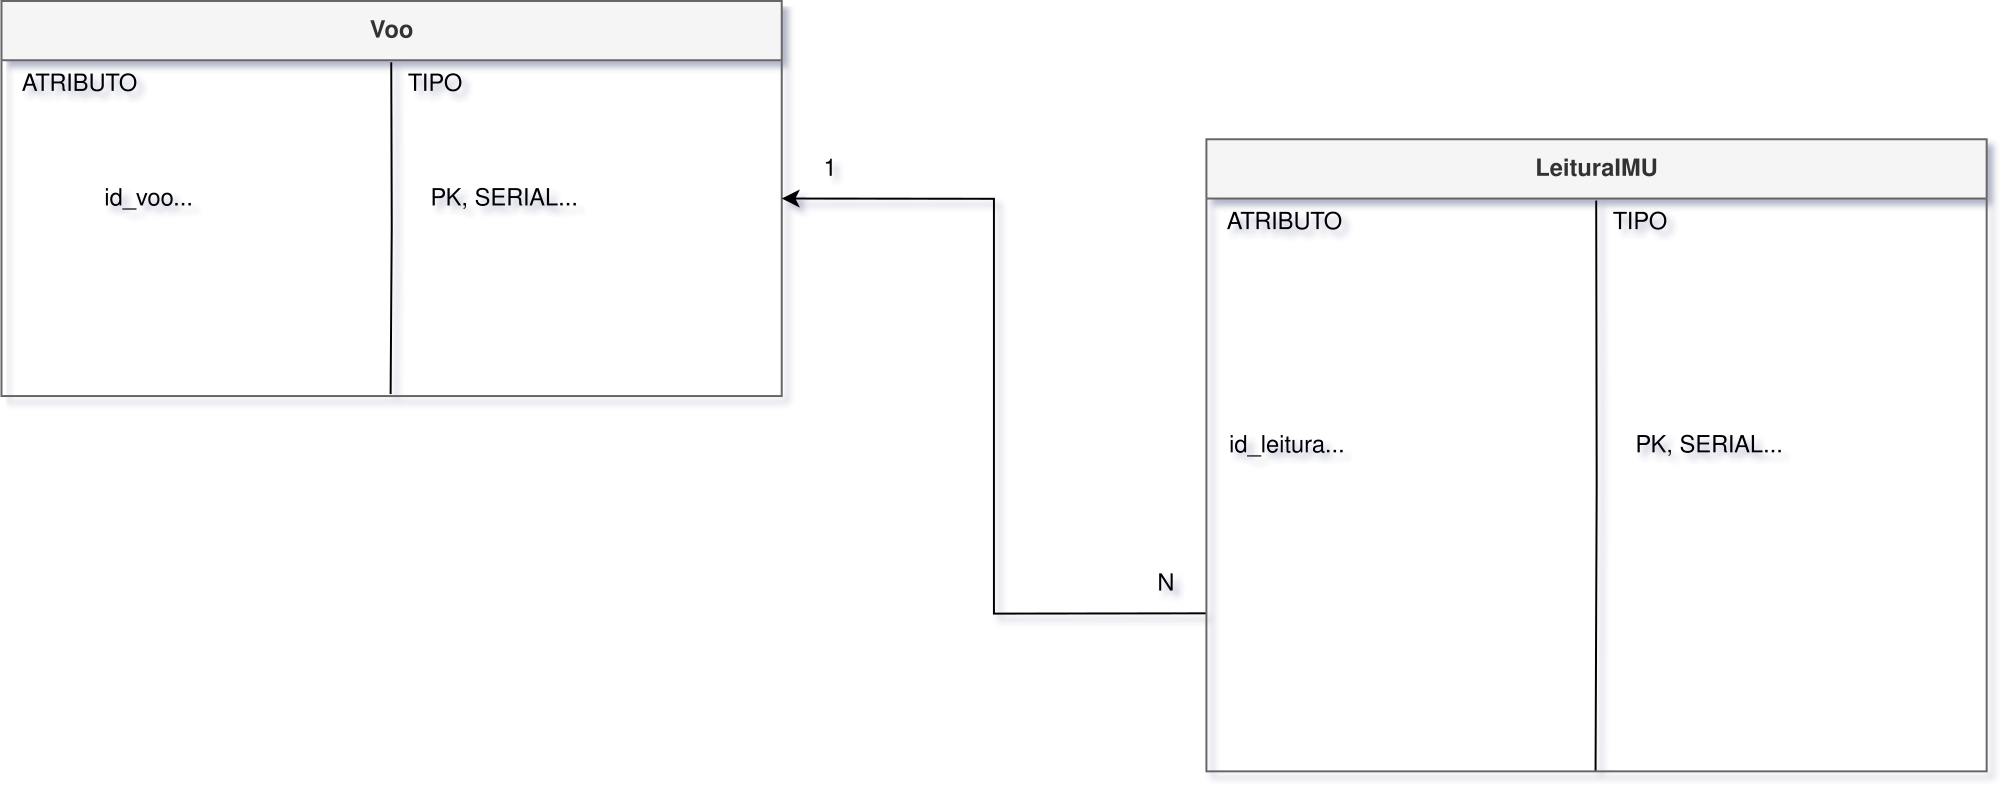
\includegraphics[width=15cm]{figuras/atributos.png}
	\caption{Pacote de Trabalho 1.3 – Atributos das Entidades}
	\label{fig_atributos}
\end{figure}

\end{samepage}

% -------------------------------------------------------------
% ARQUITETURA DO SOFTWARE
% -------------------------------------------------------------

% \section{Estilo Arquitetural}

% \subsection{Padrão Adotado: Monolítico}

\begin{samepage}

\begin{figure}[!h]
	\centering
	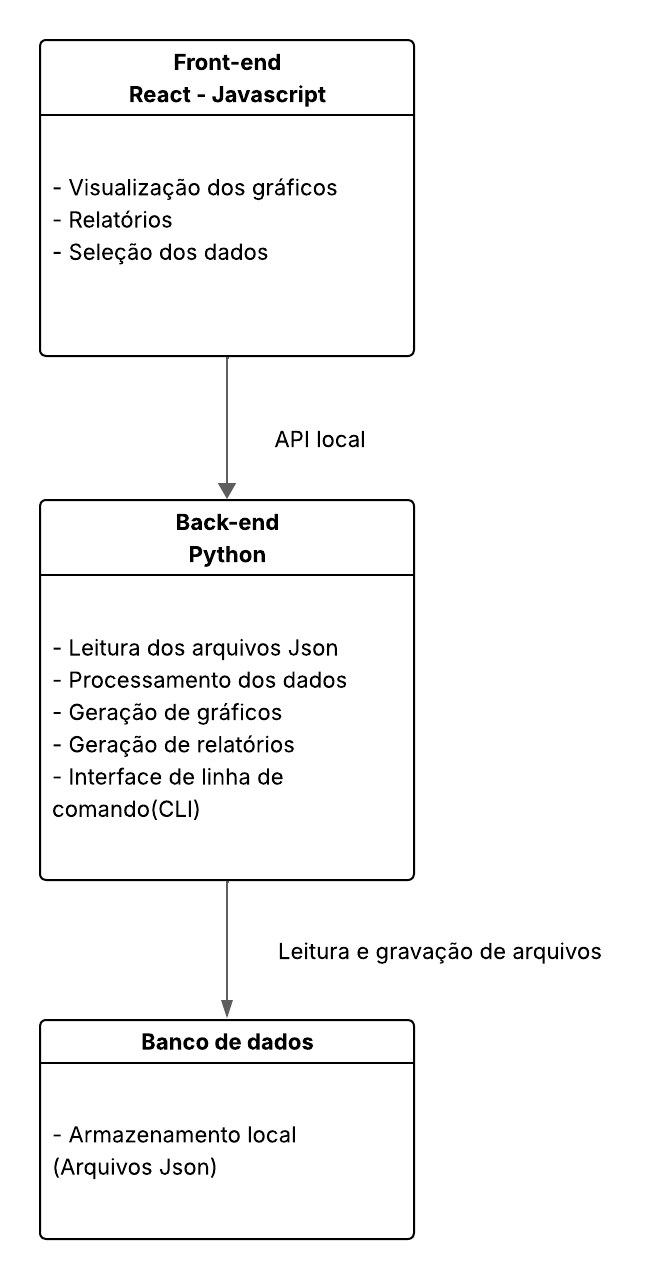
\includegraphics[width=0.75\textwidth,height=0.5\textheight,keepaspectratio]{figuras/arquitetura.png}
	\caption{Arquitetura do Software}
	\label{fig_arquitetura}
\end{figure}

O padrão arquitetural escolhido é o Monolítico, por se tratar de um sistema simples, com poucos módulos e baixa complexidade. A adoção de uma arquitetura mais robusta, como microsserviços, não se justifica neste contexto, uma vez que todo o processamento ocorre localmente e o software não possui dependências distribuídas. 

A arquitetura monolítica permite concentrar todas as funcionalidades como leitura de dados, processamento, geração de relatórios e apresentação dos resultados em um único sistema, facilitando o desenvolvimento, testes e manutenção dentro dos requisitos do projeto, como visto na Figura \ref{fig_arquitetura}.


As linguagens de programação escolhidas para o desenvolvimento do software são Python e JavaScript, cada uma com suas responsabilidades específicas dentro do sistema.

Python é responsável pelo desenvolvimento do backend e da interface de linha de comando (CLI). Utilizado para processamento dos dados, geração de relatórios, análises estatísticas e manipulação dos arquivos JSON. Utilizamos as bibliotecas Pandas para manipulação e análise de dados. NumPy para cálculos matemáticos e operações com arrays. E Matplotlib para criação de gráficos e visualizações dos dados.

JavaScript é utilizado no desenvolvimento do frontend (GUI), através da biblioteca React, para apresentar visualmente os dados dos lançamentos de forma interativa e amigável.

Neste projeto, não será utilizado um banco de dados tradicional. Os dados dos lançamentos serão armazenados localmente em arquivos JSON, por se tratar de uma solução leve, simples e suficiente para o volume de dados do projeto. Cada arquivo JSON conterá os dados de um lançamento específico, organizados de forma que possam ser facilmente acessados tanto pela CLI quanto pela interface gráfica.

\end{samepage}

% -------------------------------------------------------------------------------------------------------------------------------------------
% Fim de Software
% -------------------------------------------------------------------------------------------------------------------------------------------

\subsection{Hardware}

Este pacote contempla a concepção eletrônica do sistema, incluindo a elaboração de diagramas de blocos e esquemáticos, a instalação de sensores e atuadores no foguete e na base de lançamento, além da realização de experimentos de hardware e de integração. Envolve também a documentação técnica e a avaliação do desempenho dos fornecedores, conforme Figura \ref{fig_eap_hardware}.


\begin{figure}[!h]
	\centering
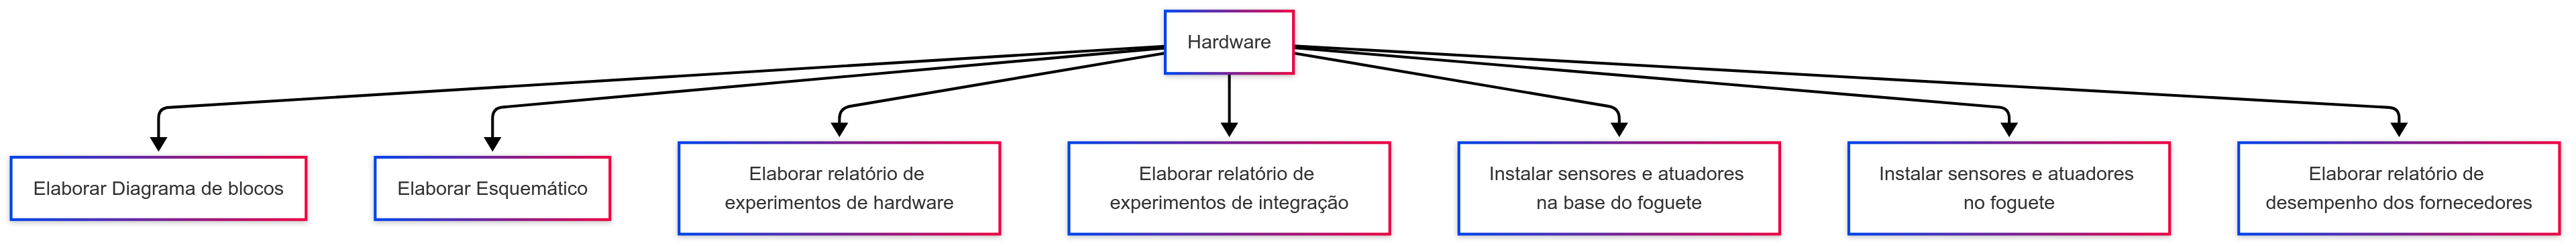
\includegraphics[width=15cm]{figuras/eap_hardware.png}
	\caption{Pacote de Trabalho 1.4 – Hardware}
	\label{fig_eap_hardware} 
\end{figure}
%\subsubsection{Objetivo do Hardware}

O objetivo principal do hardware é fornecer os meios eletrônicos e físicos para coletar os dados necessários para o controle de trajetória do foguete d'água e para automatizar o processo de lançamento. Isso envolve a integração de sensores para medir parâmetros como pressão, ângulo, altitude, velocidade e aceleração.

O hardware é projetado para trabalhar em conjunto com o software, onde os dados coletados pelos sensores são processados e utilizados para analisar trajetória do foguete. A escolha dos componentes de hardware é feita para garantir que eles atendam aos requisitos de desempenho do software, como a precisão das medições e a armazenar os dados.

\textbf{Implementação do Hardware}

Para cumprir o objetivo de coletar dados de voo e controlar o sistema de lançamento, o hardware é implementado utilizando o microcontrolador ESP32 como o componente central de processamento. O desenvolvimento do código para o ESP32 será realizado na Arduino IDE (Integrated Development Environment), uma plataforma de desenvolvimento integrada que simplifica significativamente o processo de escrita, compilação, upload e depuração do código para microcontroladores. A escolha da Arduino IDE se deve à sua facilidade de uso, vasta comunidade de suporte e disponibilidade de bibliotecas, o que acelera o desenvolvimento e reduz a complexidade do projeto. A linguagem de programação utilizada será o "C", devido à sua eficiência, controle de baixo nível e adequação para sistemas embarcados onde o desempenho e o uso eficiente de recursos são críticos.

O microcontrolador ESP32 é responsável por orquestrar a coleta, o pré-processamento e o armazenamento dos dados provenientes do sensor. Para facilitar a interação com os diversos periféricos e garantir a modularidade e a reutilização do código, serão utilizadas bibliotecas específicas:

Para a comunicação com o módulo de cartão SD, será utilizada a biblioteca SD.h, que fornece um conjunto robusto de funções para leitura e escrita de dados em cartões SD no formato FAT32. Essa biblioteca permite a criação, abertura, leitura, escrita e fechamento de arquivos, bem como a manipulação de diretórios, garantindo a persistência dos dados de voo para análise posterior.

Para a leitura dos dados do sensor MPU-6500, será utilizada a biblioteca Adafruit MPU6050 (ou similar), que abstrai a complexidade da comunicação I2C com o sensor e fornece funções para a obtenção de dados de aceleração e velocidade angular em três eixos. Essa biblioteca simplifica a calibração do sensor e a conversão dos dados brutos em unidades físicas, facilitando o desenvolvimento do firmware.

O sensor MPU-6500, um componente essencial para a medição da orientação e do movimento do foguete, é instalado estrategicamente no foguete para capturar com precisão a aceleração e a velocidade angular durante o voo. Os dados coletados por este sensor são cruciais para a reconstrução da trajetória do foguete e para a análise do seu desempenho. Especificamente, o MPU-6500 fornece dados de aceleração linear nos três eixos cartesianos (x, y e z), permitindo determinar as forças que atuam sobre o foguete em cada direção, através da aplicação da segunda lei de Newton. A velocidade angular, também medida nos três eixos, é fundamental para compreender a rotação e a estabilidade do foguete durante o voo. A integração temporal dos dados de aceleração, combinada com a orientação obtida da velocidade angular, possibilita o cálculo do deslocamento do foguete ao longo do tempo, fornecendo informações detalhadas sobre a sua posição e trajetória no espaço. Simultaneamente, um módulo de leitura de cartão SD é integrado ao sistema para fornecer um meio de armazenamento local e não volátil para os dados de voo, atuando como um backup e garantindo que nenhum dado crítico se perca, mesmo em caso de falhas.

A arquitetura do firmware seguirá os princípios de sistemas de tempo real, priorizando a eficiência e o determinismo na execução das tarefas. O firmware será estruturado em um loop principal contínuo e determinístico, responsável pela execução cíclica das seguintes tarefas:

Leitura dos dados dos sensores: Os dados dos sensores, incluindo o MPU-6500, são amostrados periodicamente com uma frequência predefinida para garantir a captura adequada da dinâmica do voo.

Pré-processamento dos dados: Os dados brutos dos sensores podem ser filtrados ou convertidos em unidades físicas, se necessário, para reduzir o ruído e melhorar a precisão.

Detecção de eventos: O firmware monitora continuamente os dados dos sensores em busca de eventos significativos, como o início do lançamento, que podem ser detectados por variações bruscas na aceleração.

Armazenamento condicional dos dados: Os dados são armazenados no cartão SD apenas quando eventos significativos são detectados ou em intervalos regulares predefinidos, otimizando o uso do espaço de armazenamento e garantindo a preservação dos dados relevantes.

Essa abordagem de firmware em tempo real permite uma resposta rápida e eficiente aos eventos do voo, garantindo a coleta confiável dos dados e o controle preciso do sistema.

\begin{figure}[h!]
    \centering
    \begin{tikzpicture}[node distance=2cm,
        block/.style={rectangle, draw, minimum width=2cm, minimum height=1cm, align=center},
        cloud/.style={ellipse, draw, minimum width=2cm, minimum height=1cm, align=center},
        arrow/.style={-Stealth}
        ]

        \node (start)      [block] {Início do Loop};
        \node (read)       [block, below of=start] {Leitura dos Sensores\\(MPU-6500, etc.)};
        \node (preprocess) [block, below of=read]  {Pré-processamento\\dos Dados\\(Filtragem, etc.)};
        \node (detect)     [block, below of=preprocess] {Detecção de\\Eventos\\(Início, etc.)};
        \node (store)      [block, below of=detect]  {Armazenamento Cond.\\no Cartão SD\\(Se Evento ou Tempo)};
        \node (end)        [block, below of=store]   {Fim do Loop\\(Retorna ao Início)};

        \draw[arrow] (start)  -- (read);
        \draw[arrow] (read)       -- (preprocess);
        \draw[arrow] (preprocess) -- (detect);
        \draw[arrow] (detect)     -- (store);
        \draw[arrow] (store)      -- (end);
        %\draw[arrow] (end)        -- (start);

    \end{tikzpicture}
    \caption{Diagrama de Blocos do Firmware}
    \label{fig:firmware_diagram}
\end{figure}


\textbf{Seleção dos Componentes de Hardware}

A escolha dos componentes de hardware é baseada em objetivos específicos e na necessidade de criar um sistema coeso e eficiente.

\textbf{Microcontrolador ESP32:} Escolhido por sua capacidade de processamento e suporte para sensores e atuadores.

\textbf{Sensores (MPU-6500):} Selecionados por sua precisão e capacidade de fornecer dados confiáveis sobre o movimento do foguete.

\textbf{Módulo de cartão SD:} Selecionados por sua capacidade de armazenar dados coletados em um cartão SD, trazendo portabilidade ao sistema.

\textbf{Fonte de Energia:} Para energizar todo o sistema, será utilizada uma bateria LiPo de 1 célula (1S) com tensão de 4.2V. A alimentação será fornecida à entrada Vin de 3.3V do ESP32, que possui um regulador de tensão interno capaz de lidar com a tensão ligeiramente superior da bateria, garantindo a operação segura dos componentes.

Nesta etapa de seleção de componentes de hardware, estamos realizando uma abstração das complexidades inerentes ao fornecimento de energia para um sistema embarcado. Fatores como dimensionamento preciso da bateria, regulação de tensão para outros componentes, gerenciamento de carga/descarga, eficiência energética e dissipação de calor são considerações cruciais que impactam diretamente a estabilidade e a confiabilidade do sistema. No entanto, o detalhamento aprofundado dessas considerações, bem como a análise completa do sistema de energia, serão abordados na seção dedicada à "Energia" deste documento.

A combinação desses componentes permite a criação de um sistema de hardware robusto e eficiente, capaz de atender aos requisitos do projeto.

\begin{figure}[h!]
    \centering
    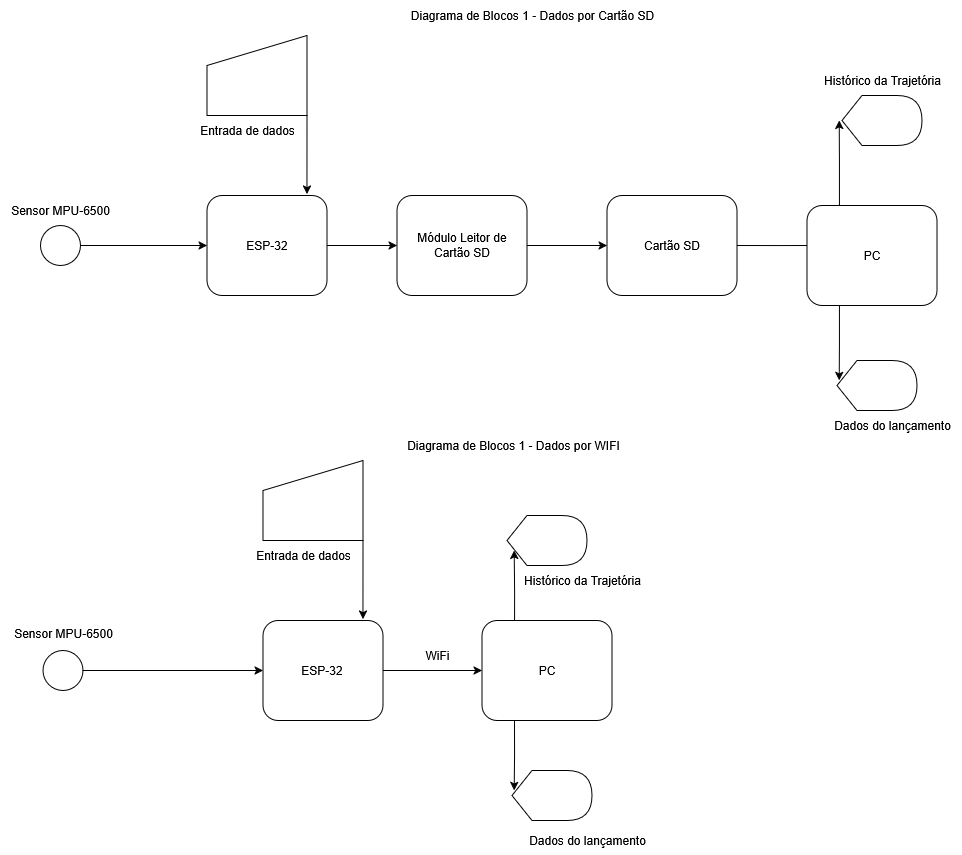
\includegraphics[width=0.8\textwidth]{figuaras/diagramaDeBlocosHardware.png}

    \caption{Diagrama de Blocos do Hardware}
    \label{fig_diagrama_blocos_hardware}
\end{figure}

\textbf{Esquemático de Conexões}

Esta seção detalha as conexões elétricas entre os componentes do sistema. É crucial observar que as informações fornecidas aqui são genéricas e podem variar dependendo dos modelos exatos dos componentes utilizados. Sempre consulte os datasheets dos componentes para obter informações precisas sobre os pinos e as especificações elétricas.

\paragraph{Representação Esquemática Básica}

A Figura \ref{fig:esquematico_basico} apresenta um diagrama esquemático simplificado das conexões entre os principais componentes do sistema.

\begin{figure}[h!]
    \centering
    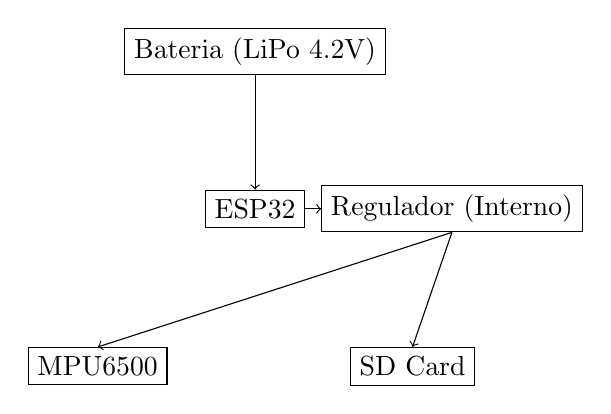
\begin{tikzpicture}
        \node[rectangle, draw] (bateria) at (0, 3) {Bateria (LiPo 4.2V)};
        \node[rectangle, draw] (esp32) at (0, 1) {ESP32};
        \node[rectangle, draw] (mpu6500) at (-2, -1) {MPU6500};
        \node[rectangle, draw] (sdcard) at (2, -1) {SD Card};
        \node[rectangle, draw] (regulador) at (2.5, 1) {Regulador (Interno)};

        \draw[->] (bateria.south) -- (esp32.north) node[midway, left] {};
        \draw[->] (esp32.east) -- (regulador.west) node[midway, above] {};
        \draw[->] (regulador.south) -- (mpu6500.north) node[midway, left] {};
        \draw[->] (regulador.south) -- (sdcard.north) node[midway, right] {};
    \end{tikzpicture}
    \caption{Esquemático Básico de Conexões}
    \label{fig:esquematico_basico}
\end{figure}

\paragraph{Detalhes das Conexões e Pinos}

 \textbf{Bateria LiPo (4.2V) para ESP32:}

Bateria Positivo (+) $\rightarrow$ ESP32 Vin: A entrada Vin do ESP32 aceita tensões mais altas e possui um regulador interno para fornecer a tensão de operação de 3.3V.

Bateria Negativo (-) $\rightarrow$ ESP32 GND: Todos os dispositivos devem compartilhar um terra comum para garantir o correto funcionamento do circuito.

\textbf{ESP32 para MPU-6500:}

O MPU-6500 utiliza o protocolo de comunicação I2C.

ESP32 SDA pin $\rightarrow$ MPU6500 SDA pin: O pino SDA (Serial Data) é utilizado para a transferência de dados seriais.

ESP32 SCL pin $\rightarrow$ MPU6500 SCL pin: O pino SCL (Serial Clock) é utilizado para a sincronização da transferência de dados.

ESP32 3.3V pin $\rightarrow$ MPU6500 VCC pin: O pino VCC fornece a alimentação de 3.3V necessária para o funcionamento do sensor.

ESP32 GND pin $\rightarrow$ MPU6500 GND pin: O pino GND fornece o terra para o sensor.

\textbf{ESP32 para Módulo de Cartão SD:}

O módulo de cartão SD utiliza o protocolo de comunicação SPI.

ESP32 MOSI pin $\rightarrow$ SD Card Module MOSI pin: O pino MOSI (Master Out Slave In) é utilizado para o ESP32 enviar dados para o cartão SD.

ESP32 MISO pin $\rightarrow$ SD Card Module MISO pin: O pino MISO (Master In Slave Out) é utilizado para o cartão SD enviar dados para o ESP32.

ESP32 SCK pin $\rightarrow$ SD Card Module SCK pin: O pino SCK (Serial Clock) é utilizado para a sincronização da transferência de dados.

ESP32 CS pin $\rightarrow$ SD Card Module CS pin (Chip Select): O pino CS é utilizado para selecionar o módulo de cartão SD. Este pino pode variar dependendo do módulo utilizado.

ESP32 3.3V pin $\rightarrow$ SD Card Module VCC pin: O pino VCC fornece a alimentação de 3.3V necessária para o funcionamento do módulo.

ESP32 GND pin $\rightarrow$ SD Card Module GND pin: O pino GND fornece o terra para o módulo.

\paragraph{Considerações sobre os Pinos do ESP32}

\textbf{ESP32 Vin:} A entrada Vin é projetada para aceitar tensões mais altas que 3.3V e possui um regulador de tensão interno para fornecer a tensão de operação adequada para o ESP32.

\textbf{ESP32 3.3V:} Os pinos de saída de 3.3V do ESP32 são utilizados para alimentar os sensores e o módulo de cartão SD.

\textbf{ESP32 GND:} É fundamental que todos os dispositivos no circuito compartilhem um terra comum para garantir o correto funcionamento e evitar danos aos componentes.

\textbf{ESP32 Pinos I2C:} Os pinos SDA e SCL para a comunicação I2C podem variar dependendo do modelo específico do ESP32. É comum utilizar os pinos GPIO21 (SDA) e GPIO22 (SCL), mas é essencial verificar o datasheet do seu ESP32.

\textbf{ESP32 Pinos SPI:} Os pinos MOSI, MISO e SCK para a comunicação SPI geralmente são fixos para a interface SPI principal do ESP32. No entanto, o pino CS (Chip Select) pode ser configurado em qualquer pino digital disponível.


\subsection{Energia}

Foca na análise do consumo energético do sistema, na seleção e validação da fonte de alimentação e na condução de experimentos relacionados à autonomia e estabilidade energética. Assim como nas demais frentes técnicas, inclui relatório de desempenho dos fornecedores de componentes de energia, conforme Figura \ref{fig_eap_energia}.

\begin{figure}[!h]
	\centering
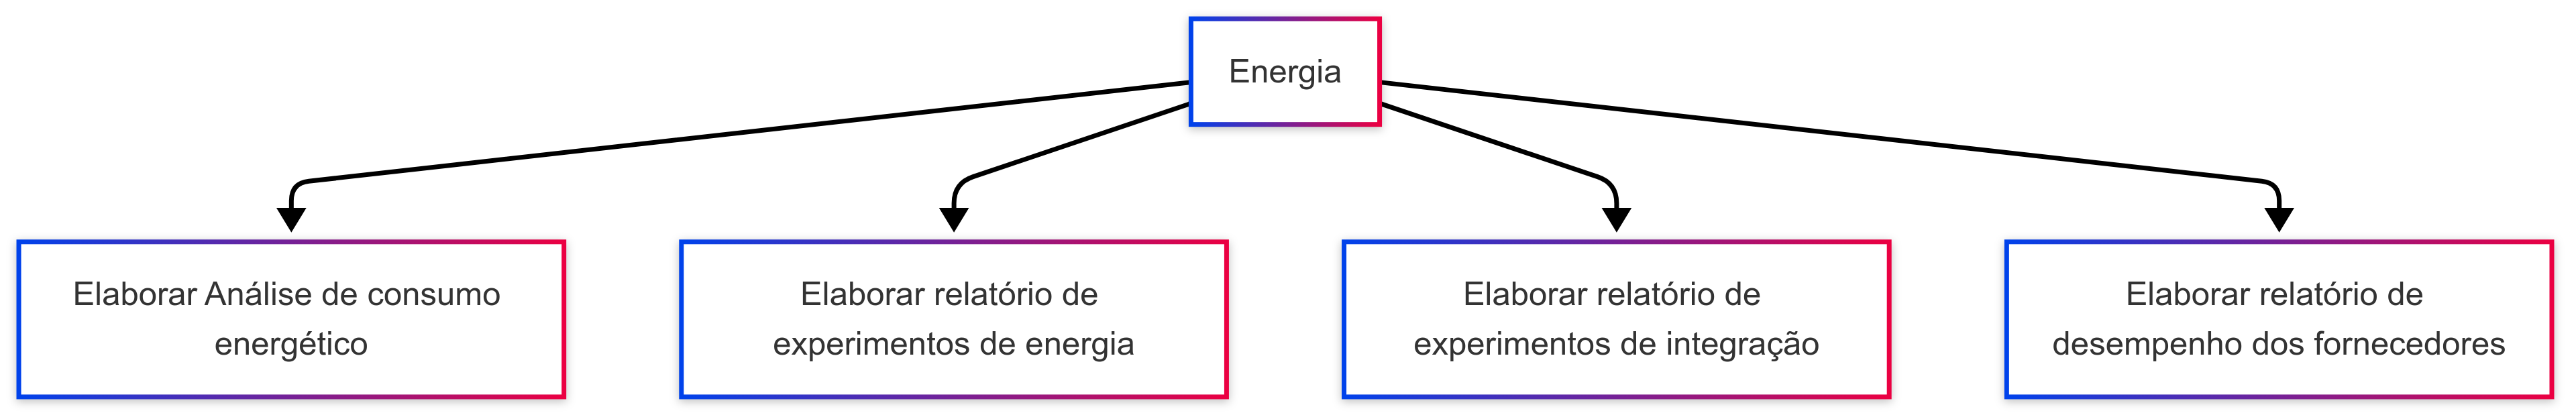
\includegraphics[width=15cm]{figuras/eap_energia.png}
	\caption{Pacote de Trabalho 1.5 – Energia}
	\label{fig_eap_energia} 
\end{figure}

\begin{figure}[h!]
    \centering
    \includegraphics[width=0.8\textwidth]{figuras/Esquematico-energia.png}
    \caption{Esquemático do Sistema de Energia}
    \label{fig_esquematico_energia}
\end{figure}

\newpage

\subsection{Integração}


Este pacote agrupa atividades de integração entre as frentes técnicas, validação dos critérios de sucesso do projeto (precisão de trajetória, reutilização, segurança), além da preparação da apresentação final e do vídeo demonstrativo. Essa fase garante que o sistema na totalidade atenda ao escopo e aos requisitos definidos, conforme representado na Figura \ref{fig_eap_integracao}.

\begin{figure}[!h]
	\centering
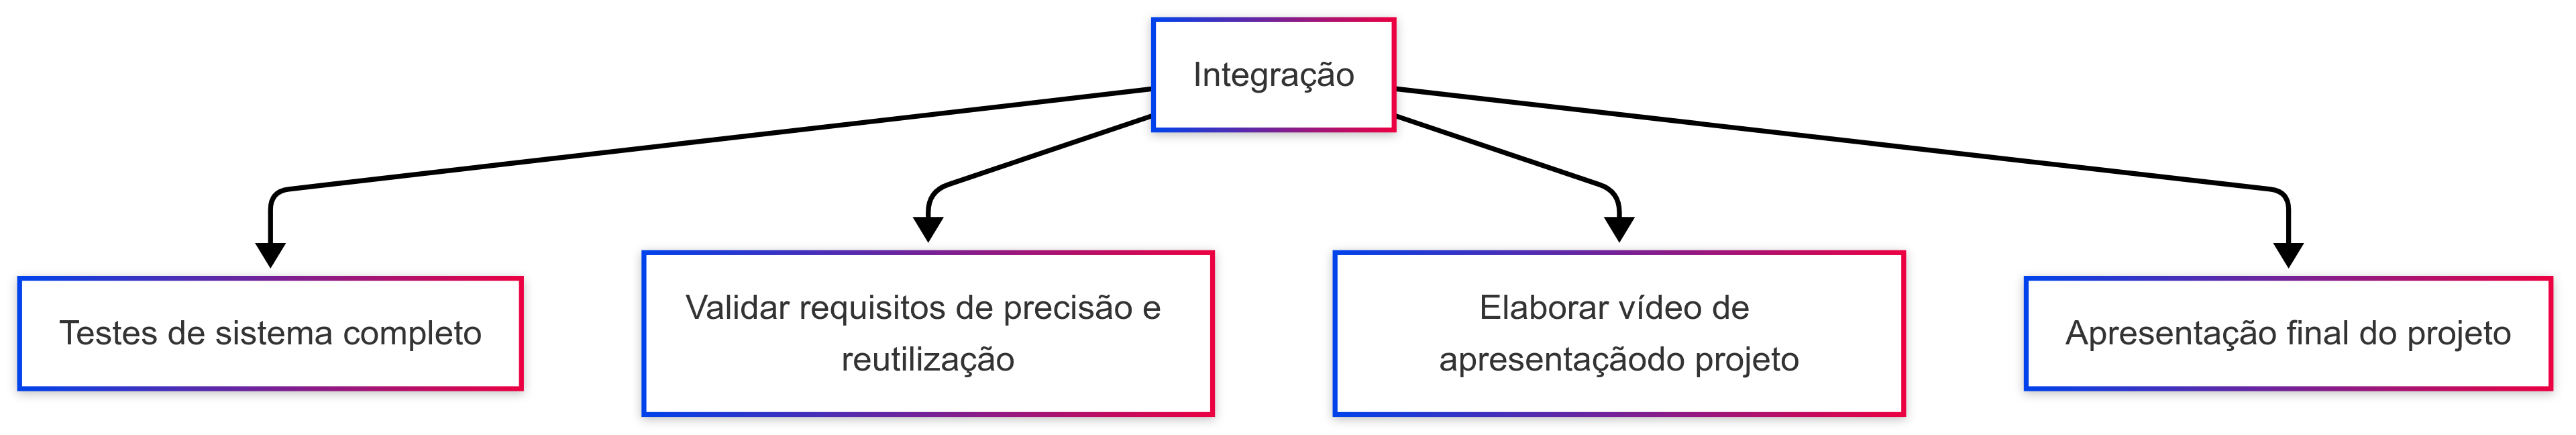
\includegraphics[width=15cm]{figuras/eap_integracao.png}
	\caption{Pacote de Trabalho 1.6 – Integração}
	\label{fig_eap_integracao}  
\end{figure}
